\section{Procedimento su HEC-HMS}
Dopo aver ottenuto la funzione della LSPP per il proprio tempo di ritorno, è possibile studiare l'analisi idrologica su HEC-HMS.\\
Per fare ciò, è necessario creare un modello idrologico per ogni bacino, in modo da immettere in input i valori pluviometrici calcolati precedentemente.\\
Il \textit{modello idrologico} è una semplificazione del fenomeno reale (nel nostro caso la trasformazione degli afflussi in deflussi).\\
Il modello idrologico, affinché possa essere soggetto della simulazione, deve avere i seguenti parametri:
\begin{itemize}
    \item bacino idrologico: indica la struttura del bacino, comprendente gli eventuali sottobacini o particolari elementi idraulici (come per esempio i canali fluviali o serbatoi);
    \item modello meteorologico: sintetizza le caratteristiche pluviometriche dell'evento meteorologico, come per esempio i bacini interessati o gli effetti ambientali del vento e dell'evapotraspirazione;
    \item specifiche di controllo: contiene le caratteristiche generali della simulazione da effettuare, come per esempio il momento di inizio e di fine;
    \item serie di dati temporali: rappresentano i valori (noti) che è possibile introdurre nel modello meteorologico, come per esempio valori pluviometrici o di deflusso. Come riportato successivamente, in questa finestra sono stati introdotti i valori pluviometrici e di deflusso reali dell'evento Vaia, in modo da calibrare il modello.
\end{itemize}
 Ulteriori proprietà, come per esempio il modello digitale del terreno, possono essere introdotti successivamente nel software.\\
 Come anticipato precedentemente, in questa relazione si andrà a studiare la risposta idrologica di due bacini, quindi risulta necessario creare due modelli di calcolo.

\subsection{Creare e calibrare il modello idrologico}
Al fine di creare un modello idrologico, e conseguentemente calibrarlo, si è scelto di studiare i bacini simulando l'evento eccezionale di Vaia del 2018.\\
In questo modo, avendo a disposizione valori certi di afflussi e deflussi, è possibile paragonare la risposta di output dal bacino che il programma calcola, con quella effettivamente misurata.\\
Questa operazione non sarebbe completamente corretta, poiché sarebbe più opportuno analizza e calibrare il bacino per eventi pluviometrici di durata maggiore a 4-5 giorni, bensì settimane o mesi.\\
Al fine di cominciare l'analisi in HEC-HMS, è necessario introdurre nel software i parametri precedentemente elencati, riferiti alla tempesta Vaia:
\begin{itemize}
    \item bacino idrologico: sono stati introdotti i file raster dei bacini (\ref{bacino_boite} e \ref{bacino_piave}) ed i valori di primo tentativo di CN e Lag time di piena (rispettivamente 35 e 270 minuti);
    \item modello meteorologico: è stata specificata la sola natura pluviometrica dell'evento, e quali bacini meteorologici incide;
    \item specifiche di controllo: si è definito il periodo interessato, che in questo caso va dal 27 ottobre 2018 al 1 novembre 2018;
    \item serie di dati temporali: sono stati introdotti i valori pluviometrici analizzati dai pluviometri di ogni sottobacino ed i valori di deflusso misurati dagli idrometri alla sezione di chiusura.
\end{itemize}

In particolare, le serie di dati temporali sono state ricavate da:
\begin{itemize}
    \item i pluviometri di Auronzo, Domegge e Santo Stefano per i relativi sottobacini del Piave;
    \item il pluviometro di Cortina, per il bacino del fiume Boite;
    \item l'idrometro del Piave, alla sua sezione di chiusura;
    \item l'idrometro del Boite, alla sua sezione di chiusura.
\end{itemize}
Dopo aver lanciato la simulazione, il cui procedimento è ampliamente riportato nel manuale ufficiale \cite{manual_hec_hms}, è possibile studiare il grafico afflussi-deflussi che il programma restituisce.\\
Il grafico riferito all'elemento in uscita dal bacino, sia questo un tratto di fiume o un punto di confluenza, possiede un solo istogramma di pioggia, ma due linee di deflusso: una riferita all'evento reale (misurato) ed una calcolata secondo i parametri di primo tentativo introdotti all'inizio (simulato).\\
Molto probabilmente, può capitare che le linee di deflusso non coincidano reciprocamente in modo sufficientemente buono; per questo motivo, risulta essenziale svolgere la \textit{calibrazione del bacino}.\\
Il processo di calibrazione del modello consiste nell'indicare al programma quali parametri del bacino andare a modificare (come per esempio il CN o il lag time), in modo che la curva del deflusso calcolato possa coincidere nel modo più ottimale possibile con quella osservata.\\
Il software, al fine di ottenere il valore ottimale, svolge una serie di calcoli iterattivi, mediante i quali analizza i parametri che l'operatore vuole che vengano migliorati.\\
Dopo aver svolto il processo di calibrazione, è possibile introdurre i parametri ottimali che il programma restituisce nel riquadro inerente alle caratteristiche del bacino; in questo modo si è a conoscenza delle caratteristiche (temporali o fisiche) che meglio approssimano quelle reali.
\begin{figure}[H]\centering
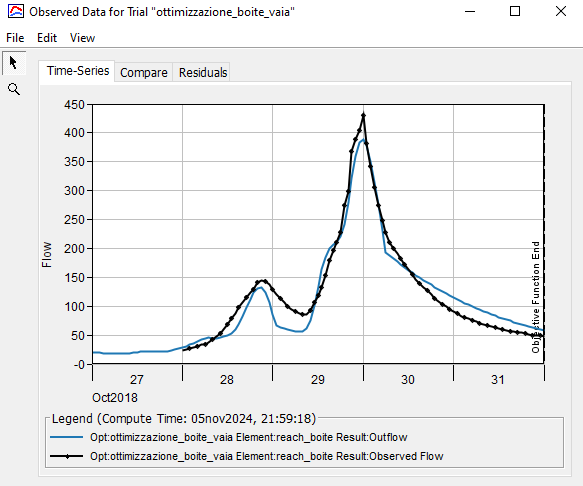
\includegraphics[scale=1]{immagini/ottim_boite.PNG}
\caption{Grafico afflussi-deflussi ottimizzato del bacino del Boite, riferito all'evento della tempesta Vaia.}
    \label{ottim_boite}    
\end{figure}

\begin{figure}[H]\centering
    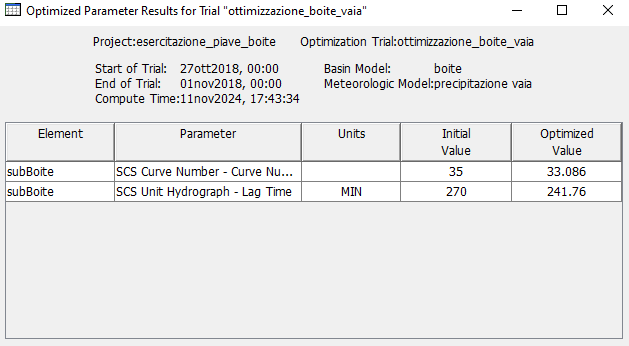
\includegraphics[scale=1]{immagini/par_ottimiz_boite.PNG}
    \caption{Parametri ottimizzati del bacino del Boite, riferito all'evento della tempesta Vaia.}
        \label{par_ottim_boite}    
    \end{figure}

In questo caso, l'algoritmo di ottimizzazione del software ritiene che i valori di CN pari a 33 e di lag time pari a 242 minuti siano quelli che fanno approssimare in modo migliore la curva di deflusso simulata del Boite rispetto a quella osservata.

\begin{figure}[H]\centering
    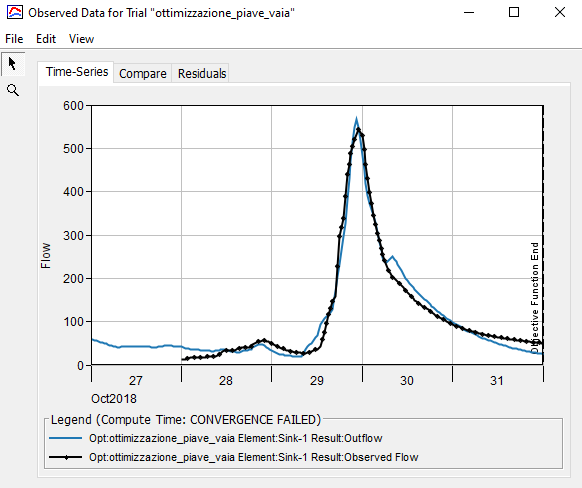
\includegraphics[scale=1]{immagini/ottim_piave.PNG}
    \caption{Grafico afflussi-deflussi ottimizzato del bacino del Piave, riferito all'evento della tempesta Vaia.}
        \label{ottim_piave}    
\end{figure}

\begin{figure}[H]\centering
    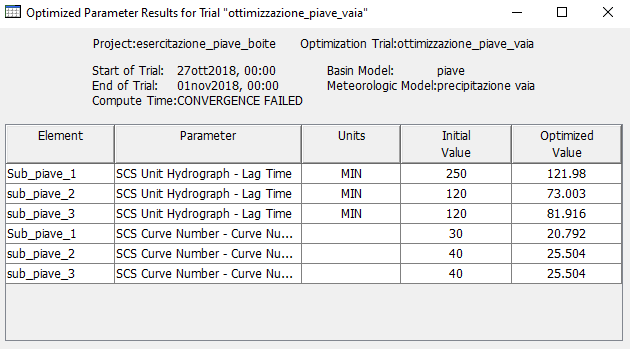
\includegraphics[scale=1]{immagini/par_ottimiz_piave.PNG}
    \caption{Parametri ottimizzati del bacino del Piave, riferito all'evento della tempesta Vaia.}
        \label{par_ottim_boite}    
    \end{figure}

Successivamente ad aver ricavato questi parametri ottimizzati, si procede a riportarli nella finestra del relativo bacino, in modo da correggere le successive simulazioni.\\
E' doveroso far presente che, i dati di CN e del Lag Time del bacino del Piave hanno dei valori insoliti, perché all'interno di esso sono presenti degli invasi, che vanno a modificare l'arrivo alla sezione di chiusura dell'acqua. Molto probabilmente, un territorio del genere, con ampie foreste di conifere e prati, può avere come valore medio un CN di 35-40.

\subsection{Applicazione del modello idrologico al proprio tempo di ritorno}
Avendo effettuato la calibrazione del modello idrologico, è possibile ripetere la medesima operazione svolta precedentemente e calcolare il volume di deflusso, data la propria precipitazione con un certo tempo di ritorno (215 anni per questa relazione).\\
Questi grafici di deflusso prendono anche il nome di \textit{idrogrammi di piena sintetici}.\\
In questo caso si andrà a creare un nuovo modello meteorologico, cercando però di simulare una precipitazione di durata simile a quella del tempo di corrivazione, in modo da massimizzare in tutti e due i casi i picchi.\\
Per questo motivo, e per quanto calcolato al capitolo sul tempo di corrivazione, si opta per imporre una durata di 12 ore al bacino del Boite e di 24 ore al bacino del Piave.

\begin{figure}[H]\centering
    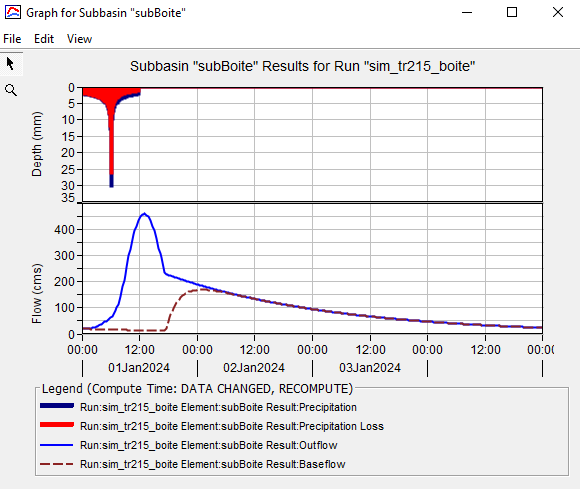
\includegraphics[scale=0.9]{immagini/boite_215.PNG}
    \caption{Grafico afflussi-deflussi del bacino del Boite, riferito ad un tempo di ritorno pluviometrico di 215 anni.}
        \label{boite_215}    
\end{figure}

\begin{figure}[H]\centering
    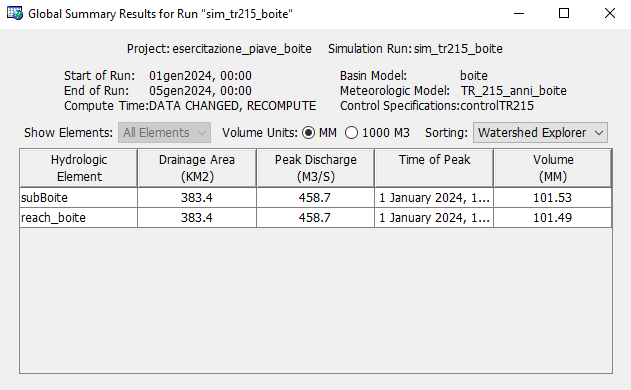
\includegraphics[scale=1]{immagini/risul_boite_215.PNG}
    \caption{Risultati dello studio dei deflussi del bacino del Boite, dato un certo tempo di ritorno.}
        \label{risul_boite_215}    
    \end{figure}

    \begin{figure}[H]\centering
        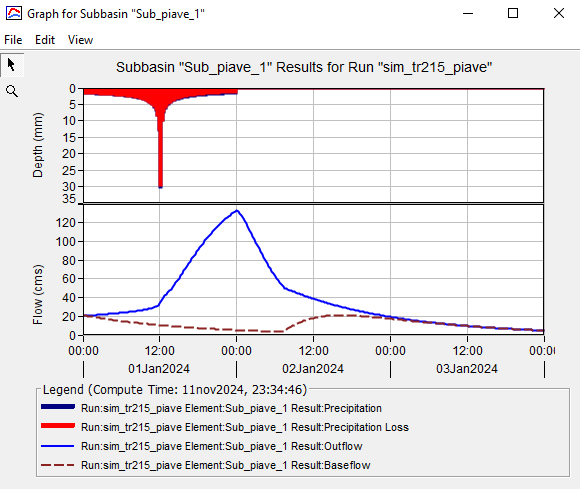
\includegraphics[scale=0.9]{immagini/sub1_piave_215.PNG}
        \caption{Grafico afflussi-deflussi del sottobacino 1 del Piave, riferito ad un tempo di ritorno pluviometrico di 215 anni.}
            \label{sub1_piave_215}    
    \end{figure}    

\begin{figure}[H]\centering
        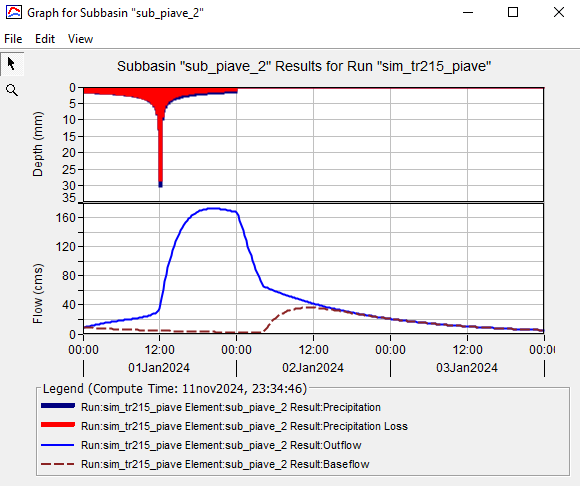
\includegraphics[scale=0.9]{immagini/sub2_piave_215.PNG}
        \caption{Grafico afflussi-deflussi del sottobacino 2 del Piave, riferito ad un tempo di ritorno pluviometrico di 215 anni.}
            \label{sub2_piave_215}    
\end{figure}
    
\begin{figure}[H]\centering
        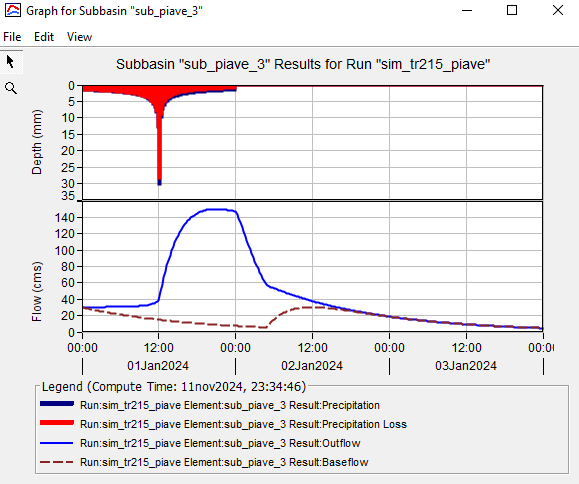
\includegraphics[scale=0.9]{immagini/sub3_piave_215.PNG}
        \caption{Grafico afflussi-deflussi del sottobacino 2 del Piave, riferito ad un tempo di ritorno pluviometrico di 215 anni.}
            \label{sub3_piave_215}    
\end{figure}    

\begin{figure}[H]\centering
    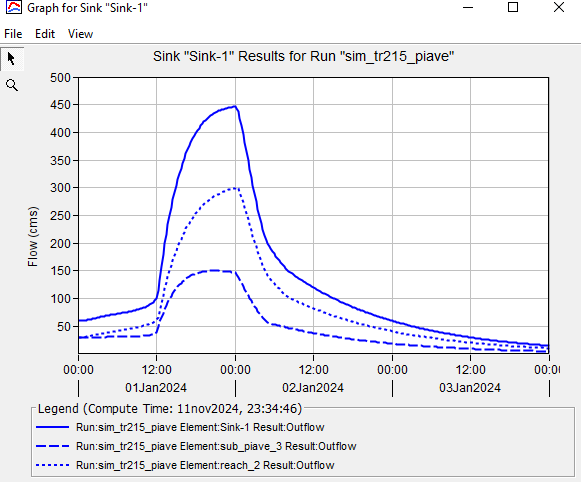
\includegraphics[scale=0.9]{immagini/sink_piave_215.PNG}
    \caption{Grafico dei deflussi totali del bacino del Piave, riferito ad un tempo di ritorno pluviometrico di 215 anni.}
        \label{sink_piave_215}    
\end{figure} 

\begin{figure}[H]\centering
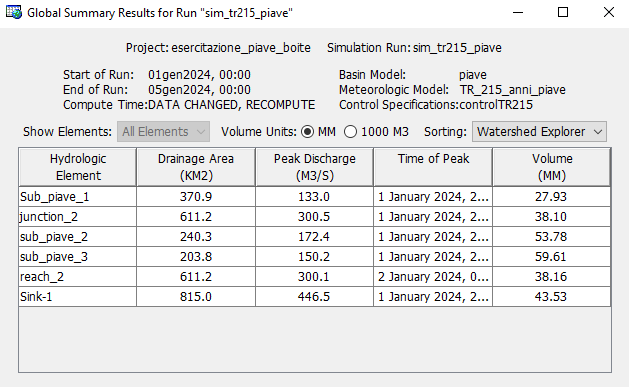
\includegraphics[scale=1]{immagini/risul_piave_215.PNG}
\caption{Risultati dello studio dei deflussi del bacino del Piave, dato un certo tempo di ritorno.}
\label{risul_piave_215}    
\end{figure}

\subsection{Analisi dei risultati ottenuti}
Dopo aver svolto i calcoli per ricavare il deflusso dei bacini, è possibile compiere alcuni ragionamenti.\\
Il bacino del Boite è interessato da una precipitazione che è di durata minore e più simile al tempo di corrivazione, rispetto a quella che si verifica nel bacino del Piave.\\
Entrambe queste caratteristiche fanno in modo che il picco di deflusso del bacino del Boite risulti molto maggiore a quello del Piave (com'è possibile verificare nelle immagini \ref{risul_boite_215} e \ref{risul_piave_215}).\\
Come anticipato precedentemente, i valori del CN del bacino del Piave sono eccessivamente ridotti rispetto a quelli reali, poiché all'interno di esso sono presenti dei bacini di immagazzinamento che fanno variare la curva di deflusso.